\documentclass{article}
\usepackage[utf8]{inputenc}
\usepackage{hyperref}
\usepackage[letterpaper, portrait, margin=1in]{geometry}
\usepackage{enumitem}
\usepackage{amsmath}
\usepackage{booktabs}
\usepackage{graphicx}
\usepackage{hyperref}
\usepackage{titlesec}
\usepackage[section]{placeins}

\hypersetup{
colorlinks=true,
    linkcolor=black,
    filecolor=black,      
    urlcolor=blue,
    citecolor=black,
}

  
\title{Economics 7103 - Homework 2}
\author{Ana Mazmishvili}
\date{ January 29, 2024 }
  
\begin{document}
  
\maketitle 

\section*{Python}
\textbf{Note:} \textit{ While working on this homework, I received assistance from Afi solely with some Python code.}

\subsection*{Question 1.1}
\textbf{Response:} Randomization worked which is demonstrated by comparison across control and treatment groups that indicates statistical balance in observables. Column 3 presents the differences in means and the standard errors of the differences in brackets. The differences are small and in case of electricity consumption statistically significant.

\begin{table}[hbt!]
    \centering
    \input{homework 2/output/table/SummaryTablePy}
    \caption{Summary Statistics for the treated and control groups.}
    \label{tab:my_label}
\end{table}


\subsection*{Question 1.2}

\begin{figure}[hbt!]
    \centering
    \includegraphics[scale = 0.7]{homework 2/output/figure/densityplotpy.pdf}
    \caption{Kernel density plots of the electricity use for treated group and control group.}
    \label{fig:hist}
\end{figure}


\FloatBarrier
\subsection*{Question 1.3}
(a) I used the Numpy package in Python to create an array X that is the 1000×4 matrix of the predictor variables (3) and a column of ones and an array Y that is the 1000×1 vector
of the dependent variable. The codes are provided in the Python code file. I used matrix operations to calculate \(\hat{\beta}\). Recall that 

\[\hat{\beta} = (X^{'}X)^{-1}X^{'}Y \]

I obtained \(\hat{\beta}\) that are presented in the first column of Table 2. 
(b) I was not able to solve this part according to your instructions. I used LinearRegression function from sklearn.linear\_model to estimate  \(\hat{\beta}\), but I did not apply Scipy.optimize.minimize() as was suggested. I do not understand this part, but I will review solutions. 

(c) I used StatsModels package to estimate \(\hat{\beta}\) and the results are presented in the third column. 


\begin{table}[hbt!]
    \centering
    \begin{tabular}{lccc}
\toprule
 & By hand & StatsModels \\
\midrule
Square feet of home & 0.620 & -83.600000 \\
=1 if house received retrofit & -109.670 & 0.620000 \\
Outdoor average temperature (\textdegree F) & 3.260 & -109.670000 \\
Constant & -83.600 & 3.260000 \\
\bottomrule
\end{tabular}

    \caption{Liniear Regression Coefficients using three approaches}
     \label{tab:beta}
  \end{table}

  


\FloatBarrier
\section*{Stata}

\subsection*{Question 2.1}

I created a table that displays each variable’s sample mean, sample standard deviation, and p-values for the two-way t-test between treatment and control group means. Please see the Table \ref{tab:sum_table}


\begin{table}[hbt!]
    \centering
    \input{homework 2/output/table/summarytable}
    \caption{Summary statistics produced using Stata}
    \label{tab:sum_table}
\end{table}

\subsection*{Question 2.2}

I created a two-way scatterplot of electricity consumption and square feet of home data using Stata. Please refer to the Figure below.

\begin{figure}[hbt!]
    \centering
    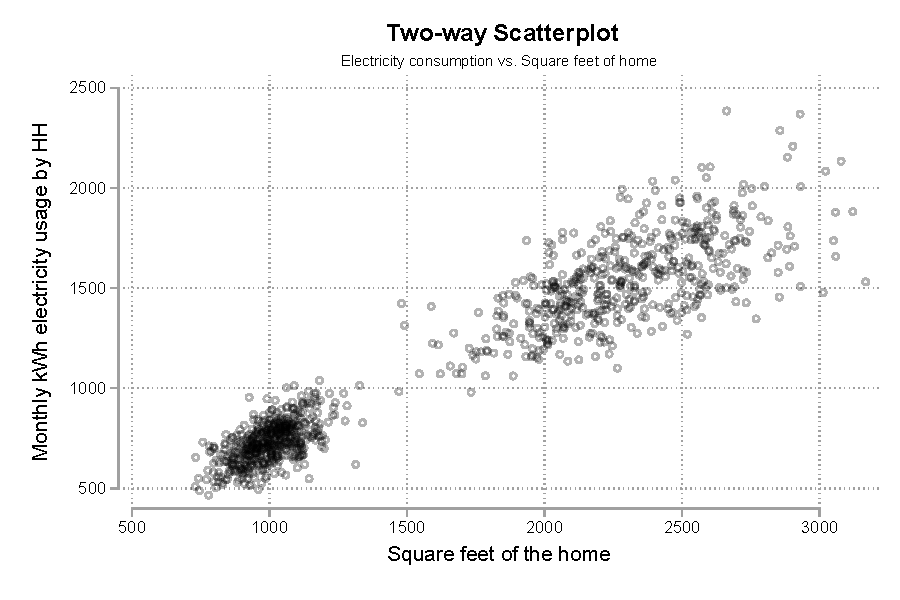
\includegraphics[scale = 0.7]{homework 2/output/figure/scatterplot.pdf}
    \caption{Scatterplot with electricity consumption and square feet of home}
    \label{tab:scatter}
\end{figure}

\FloatBarrier
\subsection*{Question 2.3}
I estimated model using OLS and obtained heteroskedasticity robust standard errors and coefficients. Please refer to the Table below. 

\begin{table}[hbt!]
    \centering
    \input{homework 2/output/table/robustOLS}
    \caption{OLS regression results using Stata}
     \label{tab:robust_table}
  \end{table}




\end{document}